\documentclass[showpacs, oneside, onecolumn, prl, amsmath, amssymb, nofootinbib, superscriptaddress, notitlepage]{revtex4-1}


\usepackage{cases}
\usepackage{amsmath}
\usepackage{amssymb}
\usepackage{amsfonts}
\usepackage{amssymb}
\usepackage{dcolumn}
\usepackage{bm}
\usepackage{bbm}
\usepackage{graphicx}
\usepackage{xcolor}
\usepackage{array}
\usepackage{subfigure}
\usepackage{hyperref}
\usepackage{multirow}
\usepackage{ulem}

%%%%%%%%%%%%%%%%%%%%%%%%%%%%%%%%%%%%%%%%%%%%%%%%%%%%%%%%%%%%%%%%%%%%%%%%%%%%%%%%%%%
\newcommand{\bra}[1]{\langle #1\vert}
\newcommand{\ket}[1]{\vert #1\rangle}
\newcommand{\nn}{\nonumber \\}
\newcommand{\lag}{\langle}
\newcommand{\rag}{\rangle}
\newcommand{\cN}{{\cal N}}
\newcommand{\cA}{{\cal A}}
\newcommand{\gsim}{\mathrel{\hbox{\rlap{\lower.55ex \hbox {$\sim$}}
                   \kern-.3em \raise.4ex \hbox{$>$}}}}
\newcommand{\lsim}{\mathrel{\hbox{\rlap{\lower.55ex \hbox {$\sim$}}
                   \kern-.3em \raise.4ex \hbox{$<$}}}}

\newcommand\be{\begin{equation}}
\newcommand\ba{\begin{align}}
\newcommand\bas{\begin{align*}}
\newcommand\bt{\begin{table}}
\newcommand\bts{\begin{table*}}
\newcommand\bfig{\begin{figure}}
\newcommand\bfs{\begin{figure*}}
\newcommand\ee{\end{equation}}
\newcommand\ea{\end{align}}
\newcommand\et{\end{table}}
\newcommand\ets{\end{table*}}
\newcommand\efig{\end{figure}}
\newcommand\efs{\end{figure*}}
\newcommand\RA{$\ \ \Rightarrow\ \ $}


\newcommand\blue{\textcolor{blue}}
\newcommand\gray{\textcolor{gray}}
\newcommand\green{\textcolor{teal}}
\newcommand\red{\textcolor{red}}




\hypersetup{colorlinks=true,
            breaklinks=true,
            pdfstartview=Fit,
            linkcolor=blue,
            citecolor=green,
            urlcolor=blue}

\bibliographystyle{apsrev4-1}




%%%%%%%%%%%%%%%%%%%%%%%%%%%%%%%%%%%%%%%%%%%%%%%%%%%%%%%%%%%%%%%%%%%%%%%%%%%%%%%%%%%
\begin{document}
	
\title{Problem Set 5}


\author{JIAO Hao}


%%%%%%%%%%%%%%%%%%%%%%%%%%%%%%%%%%%%%%%%%%%%%%%%%%%%%%%%%%%%%%%%%%%%%%%%%%%%%%%%%%%


\maketitle

%%%%%%%%%%%%%%%%%%%%%%%%%%%%%%%%%%%%%%%%%%%%%%%%%%%%%%%%%%%%%%%%
\section{Problem 1}

%%%%%%%%%%%%%%%%%%%%%%%%%%%%%%%%%%%%%%%%%%%%%%%%%%%%%%%%%%%%%%%%
\section{a)}

\textbf{Describe in comments how you go about doing this:}

Fistly, get the data of Livingston and Hanford:

{\color{gray}
%~~~~

dic='LOSC\_Event\_tutorial/LOSC\_Event\_tutorial/'}

Here we only consdier the LOSC\_4\_V2-1126259446-32.hdf5 for Livingston and Hanford. The other three events are similar.

{\color{gray}

\# the files are in the same folder

~~~~

\# Livingston noise model

fnameL='L-L1\_LOSC\_4\_V2-1126259446-32.hdf5'

strainL,dtL,utcL=rl.read\_file(dic+fnameL)

\# Hanford noise model

fnameH='H-H1\_LOSC\_4\_V2-1126259446-32.hdf5'

strainH,dtH,utcH=rl.read\_file(dic+fnameH)

~~~~

template\_name='GW150914\_4\_template.hdf5'

th,tl=rl.read\_template(dic+template\_name)

~~~~}

We assume that the noise model is the square of the abs of the Fourier transformation of data (power spectrum), i.e. $N=np.abs(dft)**2$. I get the noise model (and windowed FT(strian)) by a function. But we also need to smooth and window this PS, the two operation are done by two function named ``smooth(a,npix,kind='boxcar')' and `window(a,win\_type='cos')', which list below.

The codes are:

{\color{gray}
%~~~~

def noise\_model(strain,win\_type='tukey',npix=5):

~~~~strain\_win=window(strain,win\_type=win\_type)

~~~~sft\_win=np.fft.rfft(strain\_win)

~~~~N=np.abs(sft\_win)**2

~~~~N=smooth(N,npix)

~~~~return N,sft\_win

~~~~}

\textbf{how you smooth the power spectrum and how you deal with lines (if at all)}

I smooth the power spectrum by the function I defined.

{\color{gray}
def window(a,win\_type='tukey'):

~~~~n=len(a)

~~~~x=np.linspace(-1,1,n)

~~~~if win\_type=='cos':

~~~~~~~~win=0.5+0.5*np.cos(np.pi*x)

~~~~if win\_type=='welch':

~~~~~~~~win=1-x*x

~~~~if win\_type=='tukey':

~~~~~~~~win=np.ones(n)

~~~~~~~~for i in range(n):

~~~~~~~~~~~~if np.abs(x[i])>0.5:

~~~~~~~~~~~~~~~~win[i]=0.5+0.5*np.cos(2*np.pi*(np.abs(x[i])-0.5))

~~~~return win*a

~~~~}

Then, about how to deal the line: The lines are the photon shot noise and will affect the detection og GWs.

To remove the line of data, we need to whiten the data in Fourier space. Here I use the function whiten:

{\color{gray}
def whiten(sft,N):~~~~\# sft \& N are in Fourier space

~~~~n=len(N)

~~~~white\_ft=sft/np.sqrt(N)

~~~~return np.fft.irfft(white\_ft)
}

I don't know how to remove the line in the noise power spectrum. But in the `LOSC\_Event\_tutorial', they make an analytic approximation.
%%%%%%%%

\textbf{Explain how you window the data}

I use the function below to window the data (and template if need).

{\color{gray}
def smooth(a,npix,kind='boxcar'):

~~~~aft=np.fft.fft(a)

~~~~if kind=='boxcar':

~~~~~~~~vec=np.zeros(len(a))

~~~~~~~~vec[:npix]=1

~~~~~~~~vec[-npix+1:]=1

~~~~~~~~vec=vec/np.sum(vec)

~~~~vecft=np.fft.fft(vec)

~~~~return np.fft.ifft(vecft*aft,len(a))

~~~~
}

\bfig
	\centering
	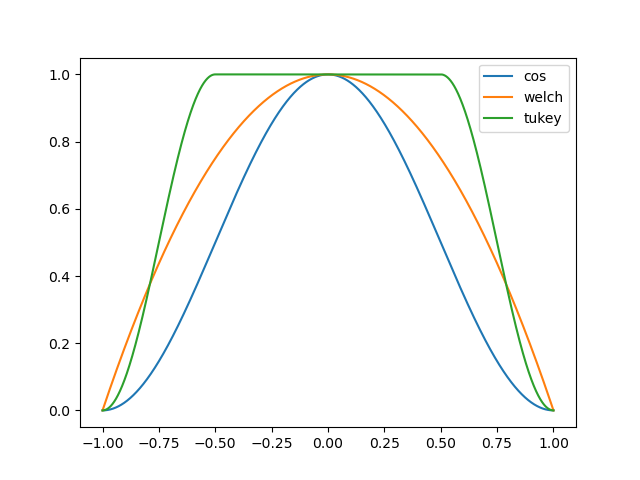
\includegraphics[scale=0.85]{5-1window.png}
	\caption{Window function of the three type I use.}
	\label{window}
\efig

Here I set 3 kinds of window function, and they are shown in fig.\ref{window}. I set `tukey' one as the default window function, which has an extended flat period near the center to avoid tapering the data/template where the signal is not small.


\bfig
	\centering
	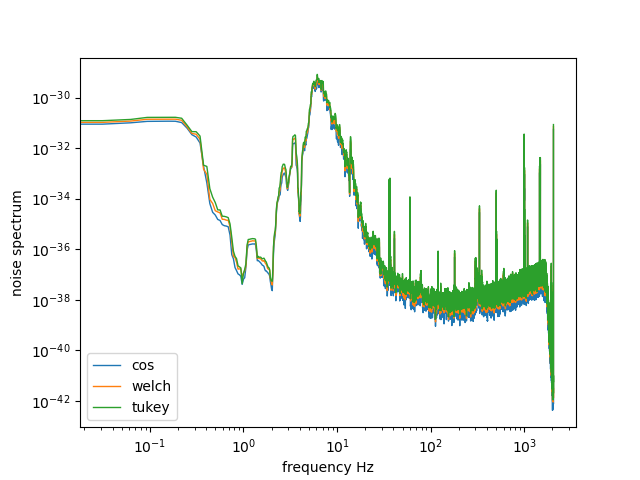
\includegraphics[scale=0.85]{5-1PS_H.png}
	\caption{The noise power spectrum Livingston and Hanford.}
	\label{PSh}
\efig

I compared the noise PS (for Hanford) with the three window function in fig.\ref{PSh}, here I set the npix of smooth to be 5. The shape of PS in the three cases are very similar, especially for the range $20Hz<f<2000Hz$, so we can only use tukey window function below.


\bfig
	\centering
	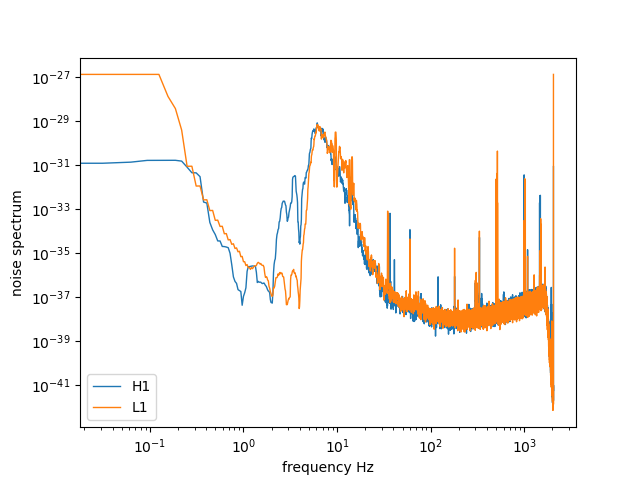
\includegraphics[scale=0.85]{5-1PS.png}
	\caption{The noise power spectrum (for Hanford) with the three window function.}
	\label{PS}
\efig

In fig.\ref{PS}, I show my noise PS for Livingston and Hanford. I use the tukey window function and set pix=5 here. The part with frequency $20 Hz<f<2000Hz/$ are simliar to the noise spectrum it should be.


\bfig
	\centering
	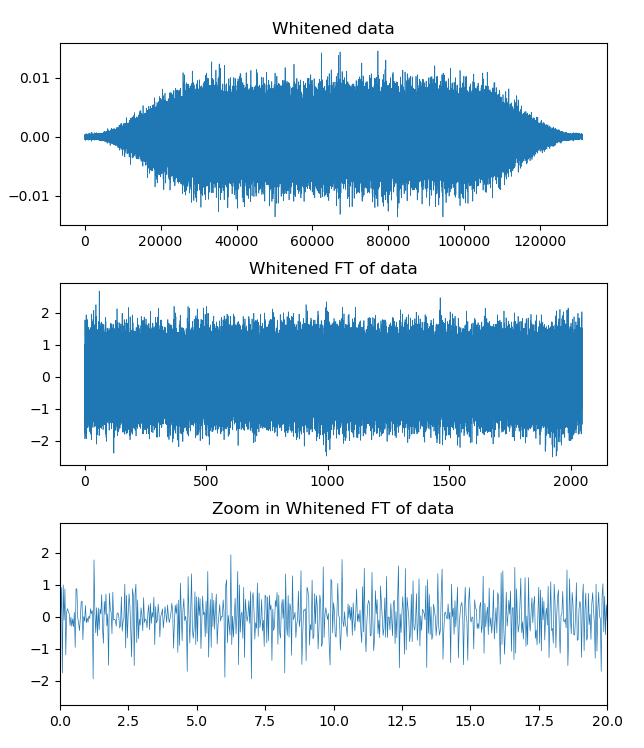
\includegraphics[scale=0.75]{5-1PW.png}
	\caption{The pre-whitened data for Hanford and it's Fourier transformation.}
	\label{5-1PW}
\efig

I also show the pre-whitened data (only H1 for example) in fig.\ref{5-1PW}. From this, we can find that tht pre-whitened data is really like whit noise (even after zooming in), so I can think my noise model is successful.


%%%%%%%%%%%%%%%%%%%%%%%%%%%%%%%%%%%%%%%%%%%%%%%%%%%%%%%%%%%%%%%%
\section{b)}

\textbf{Use that noise model to search the four sets of events using a matched filter. }

\bfig
	\centering
	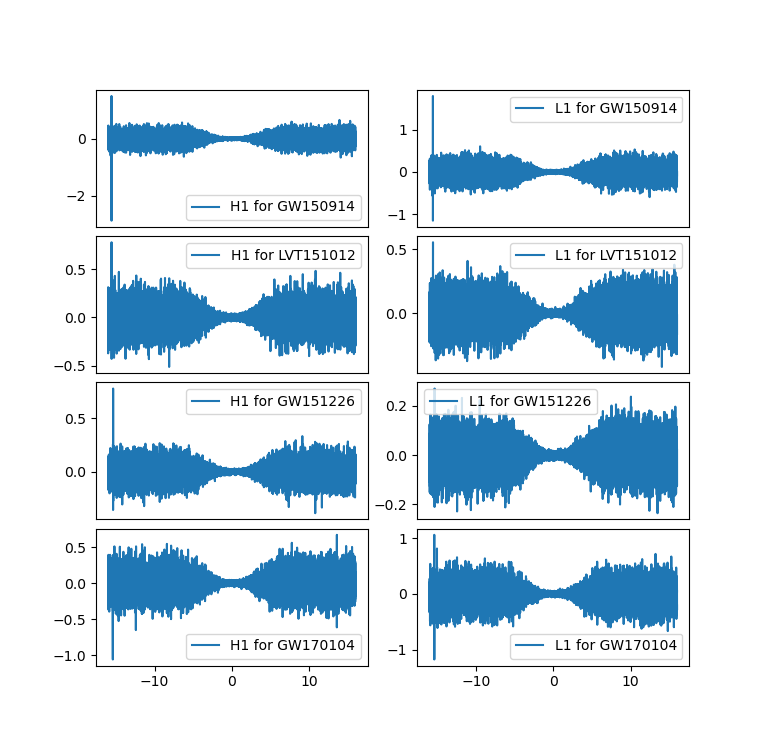
\includegraphics[scale=0.85]{5-2-1.png}
	\caption{The matched filter of the four GW events.}
	\label{5-2-1}
\efig

\bfig
	\centering
	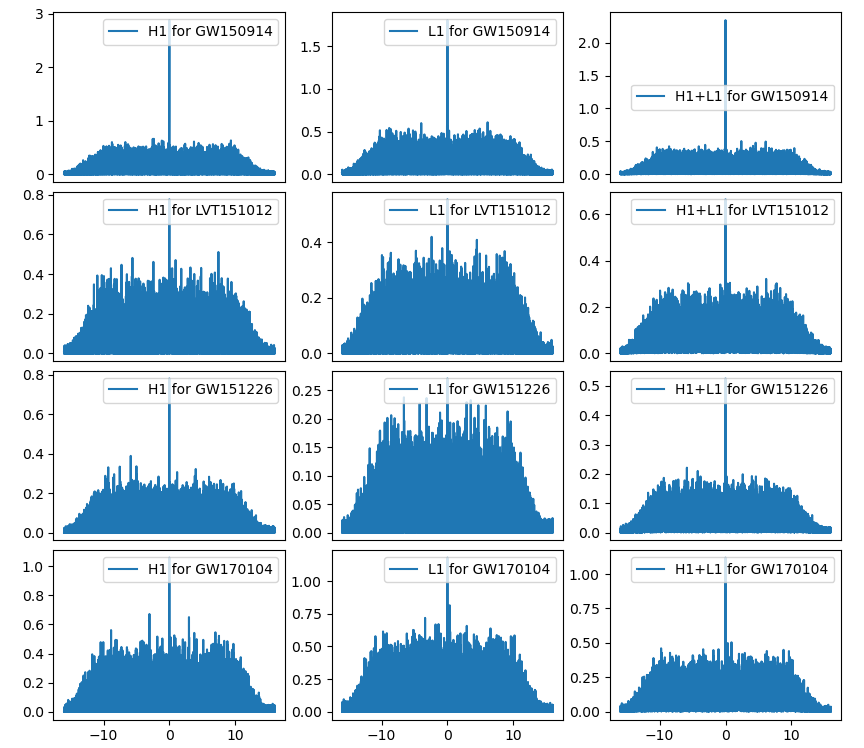
\includegraphics[scale=0.8]{5-2-2.png}
	\caption{The SNR of the four GW events.}
	\label{5-2-2}
\efig

I show the result of matched filter in fig.\ref{5-2-1}, but this fig is not very intuitive. So I shift this array to let the signal be the center, and get the abs of it, then I get the SNR (shown in fig\ref{5-2-2}). And thus, I can combine the two strains.

The position of the events and it corresponding time are listed below:

{\color{gray}
~~~~

For  GW150914 :

H1: position= 1804 , dt= 0.4404296875 s

L1: position= 1768 , dt= 0.431640625 s

~~~~

For  LVT151012 :

H1: position= 1808 , dt= 0.44140625 s

L1: position= 1816 , dt= 0.443359375 s

~~~~

For  GW151226 :

H1: position= 2653 , dt= 0.647705078125 s

L1: position= 2654 , dt= 0.64794921875 s

~~~~

For  GW170104 :

H1: position= 2490 , dt= 0.60791015625 s

L1: position= 2510 , dt= 0.61279296875 s

~~~~
}

%%%%%%%%%%%%%%%%%%%%%%%%%%%%%%%%%%%%%%%%%%%%%%%%%%%%%%%%%%%%%%%%
\section{c)}

\textbf{Estimate a noise for each event.}

Since we get the correlation matrix of these events, wecan get the noise from it. $N=diag\{\sigma_1^2,\sigma_2^2,\dots\}$, so the noise $\sigma=\sqrt{\frac1n\sum_{i=1}^n \sigma_i^2}$

{\color{gray}
~~~~

Noise for  GW150914 :

Real space:~~~~~H1: 9.614211954963066e-19 , L1: 1.0036300695958866e-16

Fourier space:	H1: 6.833523872371056e-17 , L1: 4.3141687117273126e-16

~~~~

Noise for  LVT151012 :

Real space:~~~~~H1: 2.0881871181440551e-19 , L1: 1.0442438000666774e-16

Fourier space:	H1: 6.577918949315478e-17 , L1: 4.83679095422907e-16

~~~~

Noise for  GW151226 :

Real space:~~~~~H1: 4.1818813606614847e-19 , L1: 1.0799272357994351e-16

Fourier space:	H1: 5.717579756019204e-17 , L1: 5.087493225473009e-16

~~~~

Noise for  GW170104 :

Real space:~~~~~H1: 8.340715545640844e-19 , L1: 1.3923234867196025e-16

Fourier space:	H1: 1.5934652875103644e-16 , L1: 5.975656454395538e-16

~~~~
}

I am not sure which space we should deal with the noise. Logically, The noise should be in real space, but there are many cases we should process data in Fourier space.

The noise of L1 is much larger (in real space), I think this is because the large PS at low frequency: at real space, signals at low frequency contribut a lot.

~~~~

\textbf{Signal-to-noise ratio for each event, both from the individual detectors, and from the combined Livingston + Hanford events.}

The result is shown below.

{\color{gray}
~~~~

For  GW150914 :

H1: 19.614101110750674 , L1: 14.130869906641603 , H1+L1: 18.853843267898483

~~~~

For  LVT151012 :

H1: 7.827119496923586 , L1: 6.252214706785256 , H1+L1: 7.821909909505554

~~~~

For  GW151226 :

H1: 11.454205650253543 , L1: 5.730358038167029 , H1+L1: 10.01981344024898

~~~~

For  GW170104 :

H1: 8.646809575446945 , L1: 7.651803635453794 , H1+L1: 8.939790504183573

~~~~
}

From this, we can see that the SNR of the combined data are approximate to the higher SNR of H1 and L1.

%%%%%%%%%%%%%%%%%%%%%%%%%%%%%%%%%%%%%%%%%%%%%%%%%%%%%%%%%%%%%%%%
\section{d)}

\textbf{Compare the signal-to-noise you get from the scatter in the matched filter to the analytic signal-to-noise you expect from your noise model.}

The analytic signal-to-noise you expect from your noise model: In the slides,
\bas
SNR^2/mode=(template\ FT)^2/noise\ PS\\
\Rightarrow\ \ SNR=\sqrt{\frac1n\sum \frac{(template\ FT)^2\times mode}{noise\ PS}}
\end{align*}

{\color{gray}
~~~~

For  GW150914 :

H1:   in matched filter: 19.614101110750674 ,	analytic: 8.893690917897697

L1:   in matched filter: 14.130869906641603 ,	analytic: 8.113704217675476

~~~~

For  LVT151012 :

H1:   in matched filter: 7.827119496923586 ,	analytic: 5.58368476288873

L1:   in matched filter: 6.252214706785256 ,	analytic: 5.414611584708459

~~~~

For  GW151226 :

H1:   in matched filter: 11.454205650253543 ,	analytic: 3.8919787839224447

L1:   in matched filter: 5.730358038167029 ,	analytic: 3.1915013098962954

~~~~

For  GW170104 :

H1:   in matched filter: 8.646809575446945 ,	analytic: 7.405866375578952

L1:   in matched filter: 7.651803635453794 ,	analytic: 8.618431194112965
}

We can find that for most cases, the two SNR are very different (the analytic SNR are much smaller, except for GW170104).

I think a reason is that this SNR did not use matched filter to find the best fit position of the GW event, so the SNR is much smaller.


~~~~

~~~~

%%%%%%%%%%%%%%%%%%%%%%%%%%%%%%%%%%%%%%%%%%%%%%%%%%%%%%%%%%%%%%%%
\section{e)}

\textbf{From the template and noise model, find the frequency from each event where half the weight comes from above that frequency and half below.}

I don't understand this question well, and don't know if my idea is right.

\bfig
	\centering
	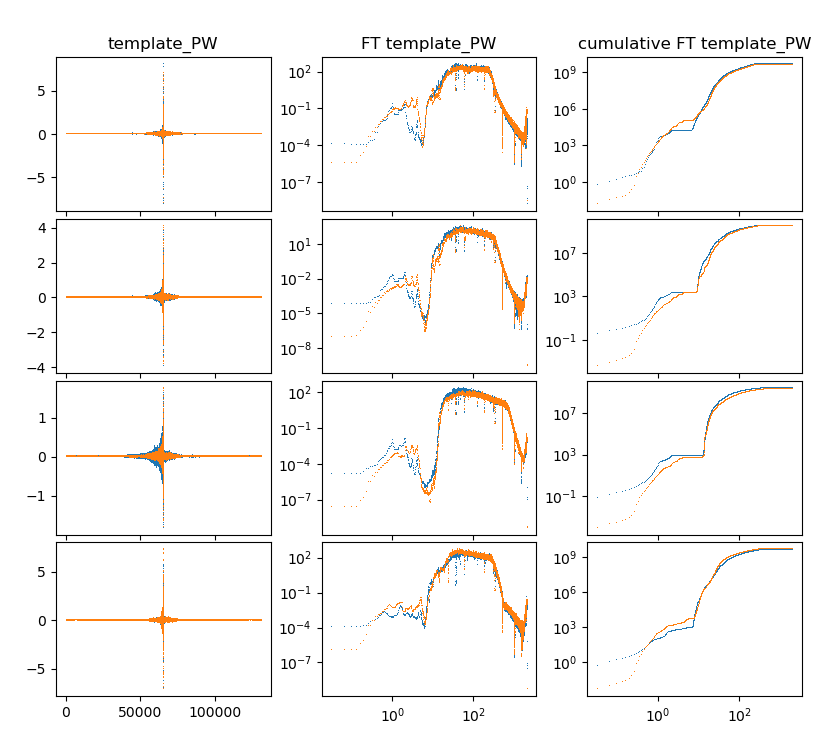
\includegraphics[scale=0.8]{5-5-1.png}
	\caption{The cumulative abs(FT(pre-whitened template)). In each penal, the blue dots denote H1 and orange dots are L1 detector. The four lines are correspond to four GW events, which are the same as above.}
	\label{5-5-1}
\efig


Assume that this frequency is the frequence at which the intergarl of abs(FT(pre-whitened template)) is the half of the total integral. To get this, we need to compute the cumulative abs(FT(pre-whitened template)), shown in fig.\ref{5-5-1}.

{\color{gray}
~~~~

The middle frequency for GW150914 :

H1: 124.40625 Hz , L1: 133.65625 Hz

~~~~

The middle frequency for LVT151012 :

H1: 113.46875 Hz , L1: 129.0 Hz

~~~~

The middle frequency for GW151226 :

H1: 130.21875 Hz , L1: 170.8125 Hz

~~~~

The middle frequency for GW170104 :

H1: 125.5 Hz , L1: 113.15625 Hz

~~~~
}


~~~~

%%%%%%%%%%%%%%%%%%%%%%%%%%%%%%%%%%%%%%%%%%%%%%%%%%%%%%%%%%%%%%%%
\section{f)}

\textbf{How well can you localize the time of arrival (the horizontal shift of your matched filter).}

The precision should be approximate to the width of the peak of matched filter.

\bfig
	\centering
	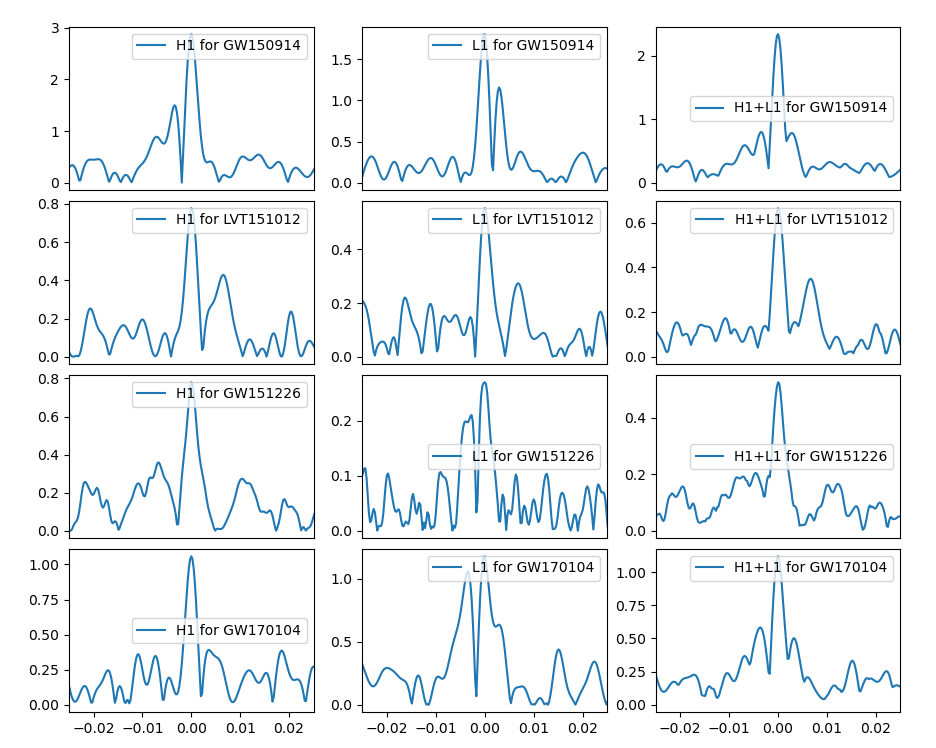
\includegraphics[scale=0.7]{5-6-1.png}
	\caption{Zooming in the matched filter of the four GW events.}
	\label{5-6-1}
\efig

Here I show the zoom in of the matched filter (still use the code of 5-2) in fig.\ref{5-6-1}.

The width of the main peak is approximately the uncertainty of the arrival time from matched filter.

From this, we can see that although the combine of the two detector won't improve the SNR, it can make the main peak much narrow, ie improve the precision of the arriving time.

I don;t know why there are two peaks of L1 matched filter for most cases. I have every steps tha same as for H1 but the result of L1 is much worse.

~~~~

\textbf{What is the typical positional uncertainy you might expect given that the detectors area a few thousand km apart?}

Since the two detector are very close (compared with the speed of GWs), the time interval of the two detector are very small. Thus, the uncertainty of the arrival time of the two detector will affect a lot.

The time interval can be get easily by the reult of 5-2.






\end{document}